\graphicspath{{./assets/}}
\setcounter{mtc}{2}
\chapter{1st Sprint: Preliminary setup of the PaaS infrastructure  }
\fancyhead[R]{\ungaramond\small\textbf{Chapter II. 1st Sprint: Preliminary setup of the PaaS infrastructure }}
\minitoc
\newpage

\section{Introduction}
In this chapter, we delve into the preliminary setup of a Platform-as-a-Service (PaaS) infrastructure, focusing on key sections that establish a solid foundation for the project.

We begin with an overview and maintenance of the existing infrastructure, gaining insight into its current state. Next, we discuss the cloud architectural design of the PaaS platform, detailing its structure and components.

Resource provisioning for the PaaS infrastructure is explored to ensure efficient allocation and management. We then cover the preliminary infrastructure setup, highlighting essential steps taken to establish a robust foundation.

Lastly, we address the initial setup of vital backend services crucial for a secure and reliable PaaS environment, including networking, load balancing, TLS provisioning, distributed storage, and authentication services.

\section{Sprint backlog :}

\begin{longtable}[ht]{|m{1.5cm}|m{3cm}|m{1.5cm}|m{8cm}|}
\hline
{\textbf{EpicID}} & {\textbf{Epic}} & {\textbf{StoryID}} & {\textbf{Story}} \\
\hline
1 &  \raggedright Exploring assets.	& 1.1  & SCM structuring: service components need to be split into different repos. \\
\cline{3-4}
& & 1.2 &  	Keeping track of developed applications and their requirements \\
\hline
2  & Maintenance. &	2.1	 &  Rebuilding optimized containers for developed applications. \\
\cline{3-4}
& & 2.2 & Backup of existing data on current infrastructure in S3 containers.\\
\hline
3  & Information gathering.	 &  3.1	 &  Research provider specific (OVH) constraints and making choices regarding orchestration, virtualized networking, load balancing and distributed storage\\
\hline
4  & \raggedright Provisioning resources using IaC playbooks and HCP config files.  &  4.1	 & Preparing provider specific(ovh) terraform config. \\
\cline{3-4}
& & 4.2 & Preparing ansible playbook to initiate provisioning. \\
\cline{3-4}
& & 4.3	& Setting up IaC host machine.  \\
\cline{3-4}
& & 4.4	& Cloud provider account and project creation.  \\
\hline
5  & Setup and configuration of provisioned resources using ansible playbooks.	 &  5.1	 &  Creating role-based assignments specific to each resource for resource setup. \\
\hline
6  & PaaS setup: Setting up the service groups for networking and storage	 &  6.1	 &  Setting up the ingress controller (traefik).\\
\cline{3-4}
& & 6.2 & Setting up the network level load balancer (metalLB). \\
\cline{3-4}
& & 6.3	& Setting up the load balancer. \\
\cline{3-4}
\hline
7  & Setting up a GitOPS compliant CI/CD workflow for the applications in development.  &  7.1	 & Setting up the CI/CD orchestrator.\\
\cline{3-4}
& & 7.2 & SCM restructuring and code adaptation. \\
\cline{3-4}
& & 7.3	& Preparing container images for the different workloads in development.  \\
\cline{3-4}
& & 7.4	& Developing GitOPS oriented pipelines for the build, scan, and deliver phases in the various environments.  \\
\cline{3-4}
\hline
\caption{1st sprint Backlog}
\end{longtable}
\newpage
\section{Overview and maintenance of the existing resources}
\subsection{Maintenance operations}

In this sprint, we have assembled standalone self-hosted services into a single stack of upgraded container versions in order to provide better visibility of workloads. A container management platform was then added to this stack to improve on operability. 
The following figure is the deployment diagram of the resulting docker-compose stack:

 \begin{figure}[H] 
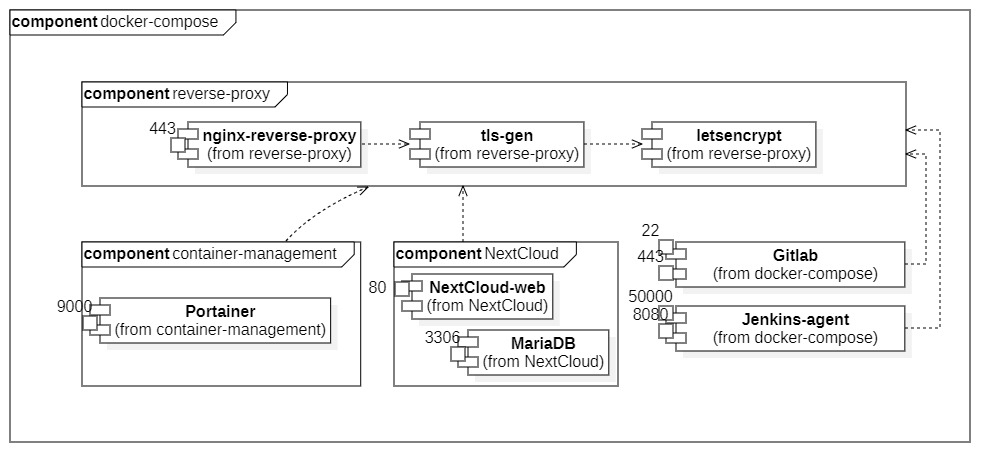
\includegraphics[width=1.0\textwidth,angle=00]{assets/f9.jpg}
\caption{PaaS infrastructure}
\label{fig:f9}
\end{figure}

The stack comprises Nginx reverse proxy for traffic routing and HTTPS encryption, a TLS generator for certificate management, Portainer for Docker container management, Nextcloud for cloud-based file sharing, GitLab for version control, and Jenkins for automation of CI/CD processes.

Each service is defined in a separate Docker container and is configured using environment variables, volumes, and ports.

This Docker Compose stack provides a scalable and easy-to-manage infrastructure for hosting multiple cloud-based services, all secured using HTTPS encryption and Let's Encrypt TLS certificates. 

\newpage

\subsection{Application overview and SCM structuring}

Two main applications were in development during this project. We have recommended a better source code management strategy that resulted in separating services into different repos in order to optimize the container image creation process. The resulting deployment diagram Is as follows: 

 \begin{figure}[H]\centering
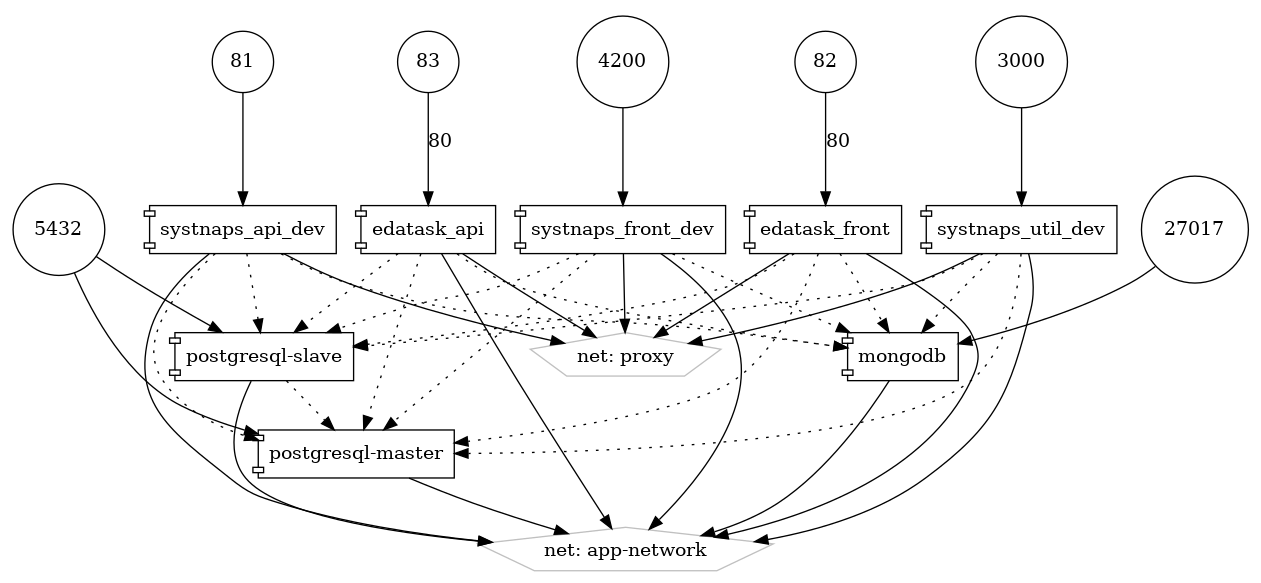
\includegraphics[width=1.0\textwidth,angle=00]{assets/f10.png}
\caption{ Deployment Diagram }
\label{fig:DeploymentDiagram}
\end{figure}

The stack includes the following services: 
\begin{enumerate}
\item Backend API: A Symfony\cite{Symfony} API that serves as the backend for the application. It is responsible for processing requests and returning data to the frontend. 
\item Frontend: An Angular\cite{Angular} web application that serves as the frontend for the application. It is responsible for displaying data and interacting with the backend API. 
\item HA PostgreSQL\cite{PostgreSQL}: A relational database management system that stores data for the application. It is used to store structured data for the backend API. 
\item Replicated MongoDB\cite{MongoDB}: A NoSQL database management system that stores data for the application. It is used to store unstructured data for the frontend. 
\item Nginx\cite{Nginx}: A web server that acts as a reverse proxy for the other services in the stack. It is responsible for routing traffic to the correct service based on the URL and handling HTTPS encryption. 
\end{enumerate}

The backend API, frontend, MongoDB and PostgreSQL are connected using the "app-network" network. All services are also connected to the "proxy" network where Nginx resides, enabling the reverse proxy detect labels and route traffic to the appropriate service based on the URL.

\newpage

\section{Cloud design of the PaaS infrastructure}
\subsection{Package diagram of cloud resources :}

The cluster resources are cloud instances with different specifications tailored to their use cases. Three major groups of resources are distinguished in the following diagram: Control plane instances, Compute instances and storage assets which are object store buckets and compute instances to which raw block stores are attached.

\begin{figure}[H]\centering
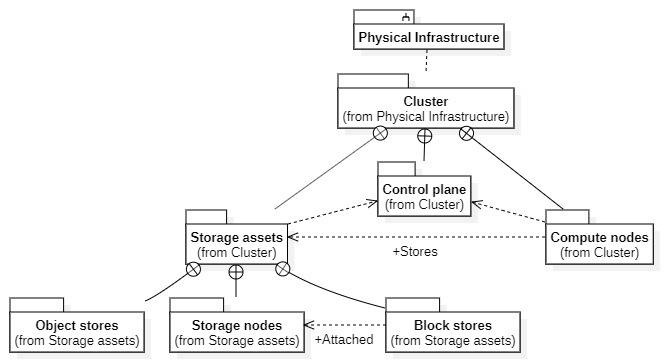
\includegraphics[width=0.74\textwidth,angle=00]{assets/f11.jpg}
\caption{Package diagram of cloud resources }
\label{fig:Package diagram of cloud resources }
\end{figure}

\subsection{Comparative study on container orchestrators: }
Container Orchestration Engines such as “Kubernetes”, “Apache Mesos” and “docker swarm” are platforms for managing containers and automating the deployment, scaling, and operations of containers across a cluster of nodes. This is achieved by pooling the discrete cloud resources into a single PaaS on which workloads can be deployed. 

\begin{longtable}[H]{|m{3.5cm}|m{3.5cm}|m{3.5cm}|m{3.5cm}|}
\hline
Criteria & Kubernetes & Docker swarm & Apache Mesos  \\
\hline
Ease of use & Medium & Easy & Complex  \\
\hline
Cluster scalability & Medium to Large & Small to Medium & Very Large  \\
\hline
Cluster installation & Complex & Easy & Medium  \\
\hline
Container deployment & YAML based  & Docker based & JSON based \\
\hline
Community Support  & Large  & Moderate  & Small \\
\hline
Configuration & Declarative  & Declarative & Imperative \\
\hline
\caption{Sprint planification}
\end{longtable}

Kubernetes is our container orchestration tool of choice in this project. It is known for its highly advanced orchestration capabilities, built-in load balancing, rolling updates, and self-healing. It has a declarative configuration model and a highly extensible architecture. However, it does have a steeper learning curve compared to Docker Swarm.  

Our goal is to tackle the task of establishing a fully sustainable PaaS by utilizing its flexibility via custom resource definitions. 

\subsection{Package diagram for the PaaS logical components:}

\begin{figure}[H]\centering
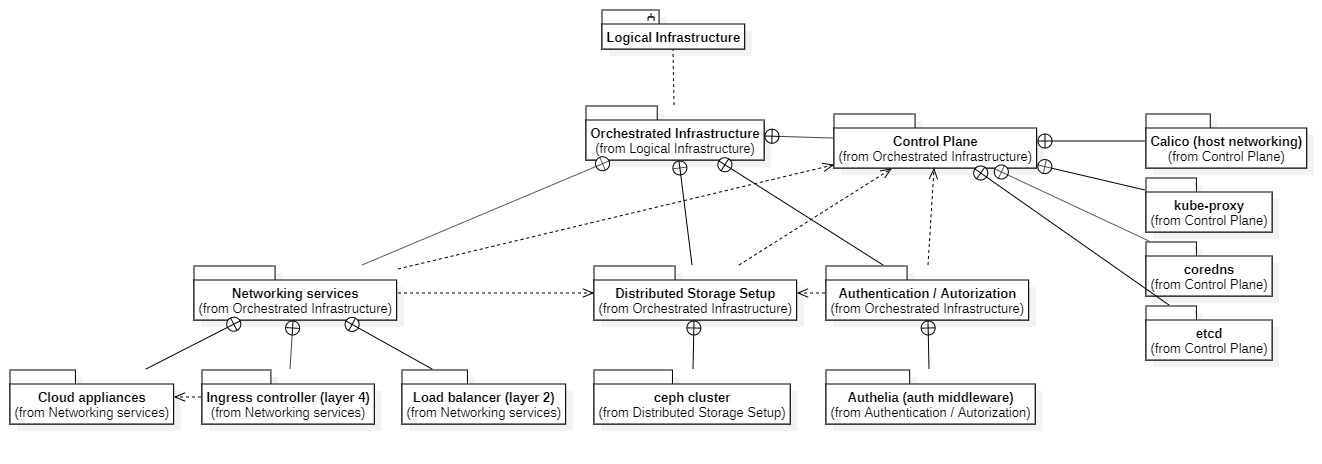
\includegraphics[width=1.0\textwidth,angle=00]{assets/f12.jpg}
\caption{Package diagram for the PaaS logical components}
\label{fig:Package diagram for the PaaS logical components}
\end{figure}

This figure illustrates a package design of the main PaaS services. We mainly distinguish: 
\begin{itemize}[label={--}]
\item  A control plane: which manages assets in the cluster, namely, nodes, pods and other api resources. 
\item An assortment of networking services which allow for ingress control in both the network and application layers. 
\item An authentication and authorization service: which is aimed to control access to the cluster. 
\item A distributed, scalable, and replicated storage backend which is independent of the infrastructure in place to provide data redundancy and disaster recovery. 
\end{itemize}
\newpage
\section{Resource provisiong for the PaaS infrastructure}
\subsection{UML design : class diagram for cloud infrastructure }
The following diagram showcases the interaction between the infrastructure as code tools and the cloud provider as well as the resulting infrastructure, its components, and the relation between them. 
\begin{figure}[H]\centering
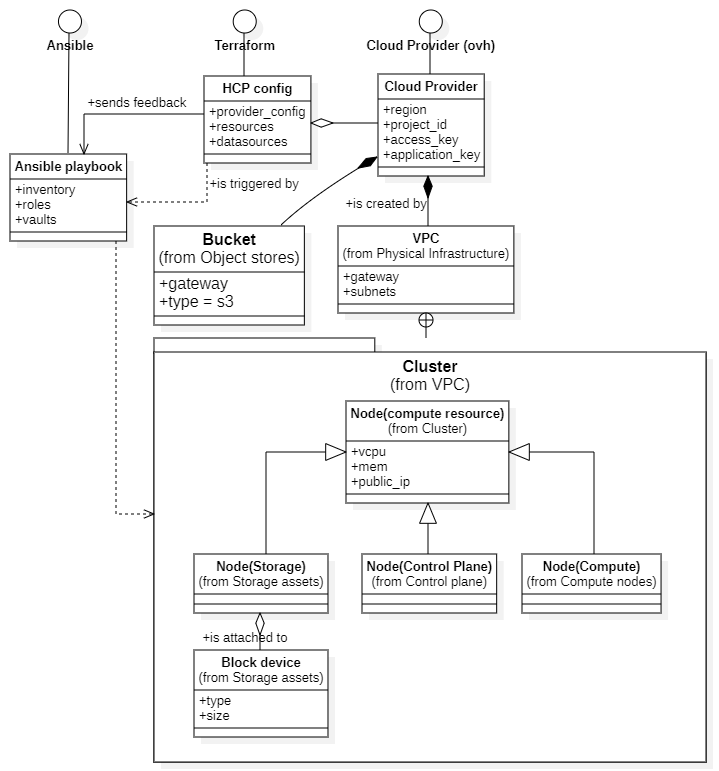
\includegraphics[width=1.0\textwidth,angle=00]{assets/f13.png}
\caption{Class Diagram for cloud infrastructure}
\label{fig:fig13}
\end{figure}

\subsection{“HCP config” diagram for cloud provisioning: }
The following figure illustrates the main resources declared in our terraform “HCP config”: 

\begin{figure}[H]\centering
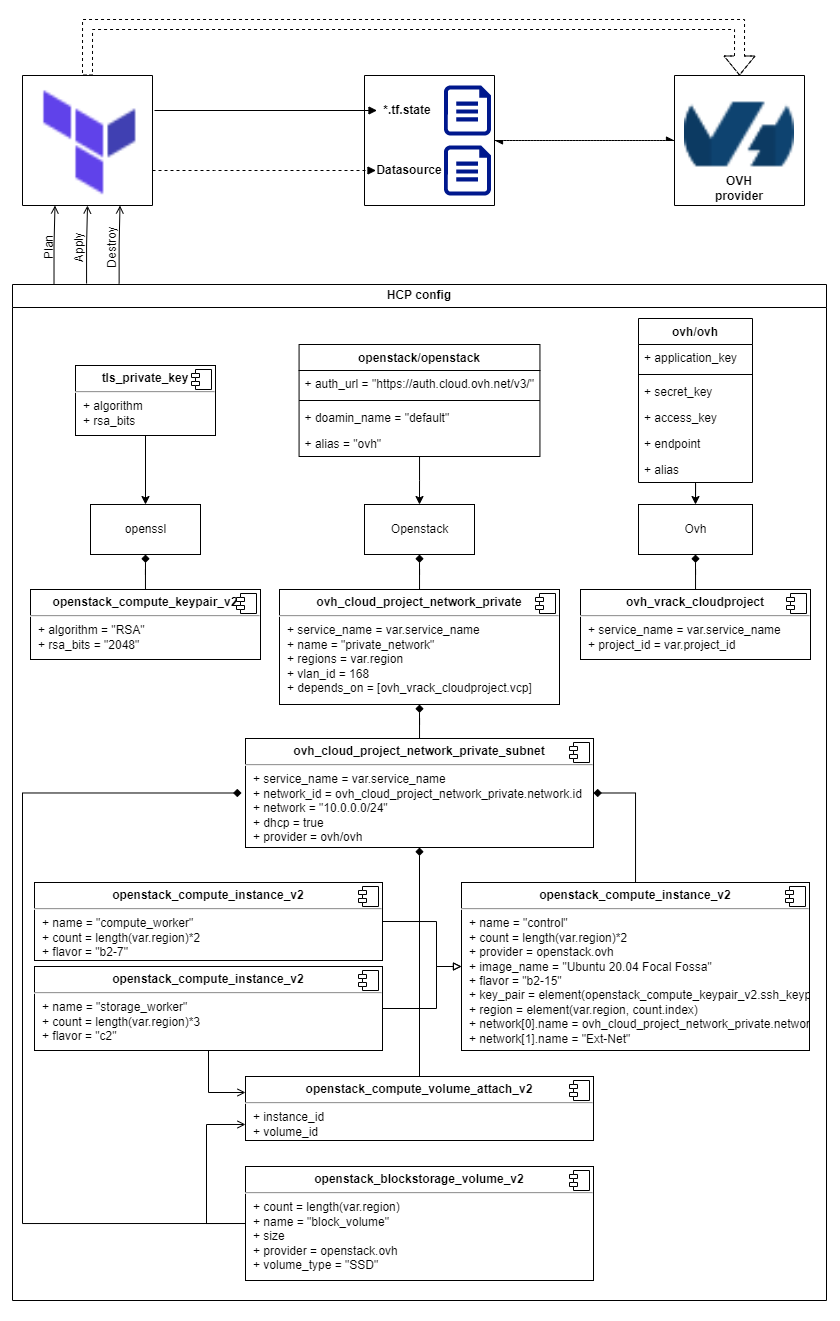
\includegraphics[width=0.8\textwidth]{assets/f14.png}
\caption{Diagram for cloud provisionning}
\label{fig:fig14}
\end{figure}
\newpage
The previous diagram shows a Terraform configuration for deploying resources on OVH cloud provider. The configuration consists of four main components: provider, network, compute, and storage. 

\begin{itemize}[label={--}]
\item The provider component specifies the OVH cloud provider and the authentication credentials to access the account. 
\item The network component defines the virtual private cloud (VPC) and its associated resources, such as subnets, security groups, and routers. 
\item The compute component defines the public cloud compute instances that will host our PaaS. The VMs are launched in the subnets defined in the network component, and their configurations are specified through variables. 
\item The storage component defines the object storage bucket that will store application and backup data, and the block storage volumes that will be attached to the VMs. 
\end{itemize}

All the resources are managed by Terraform, which allows for easy provisioning, scaling, and management of the infrastructure. 

Overall, this Terraform configuration with OVH cloud provider provides a scalable, secure, and highly available infrastructure for running applications. 

\subsection{Component diagram of provisioned resources}

\begin{figure}[H]\centering
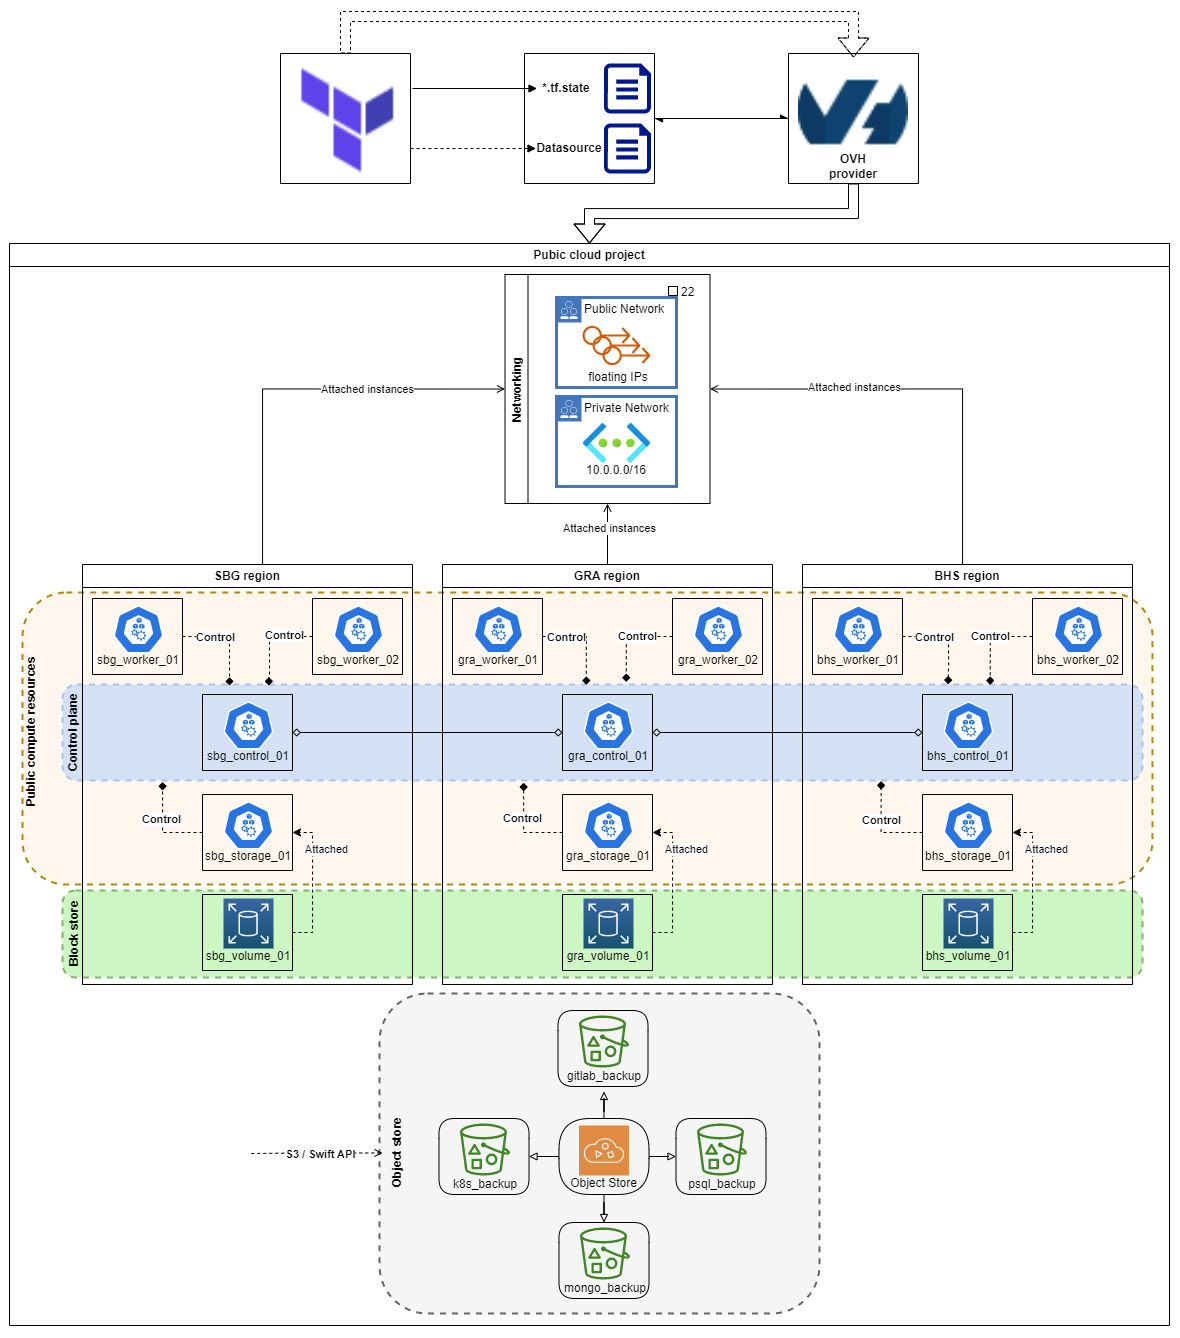
\includegraphics[width=1.0\textwidth,angle=00]{assets/f15.png}
\caption{Component diagram of provisioned resources}
\label{fig:fig15}
\end{figure}

The cluster resources were deployed to three regions. Namely, GRA, BHS, SBG. In each region, four instances were created. One of which will join the control plane, two will have the worker compute role and the last will have a second block device in raw format and will join the data storage backend. Various buckets from the object store will be provisioned and will serve as backup storage backends and high-speed data storage.

\section{Preliminary infrastructure setup}

\subsection{UML design: sequence diagram for infrastructure setup}

The following is a sequence diagram that shows the flow of actions or events that occur during the process of setting up the infrastructure.

\begin{figure}[H]\centering
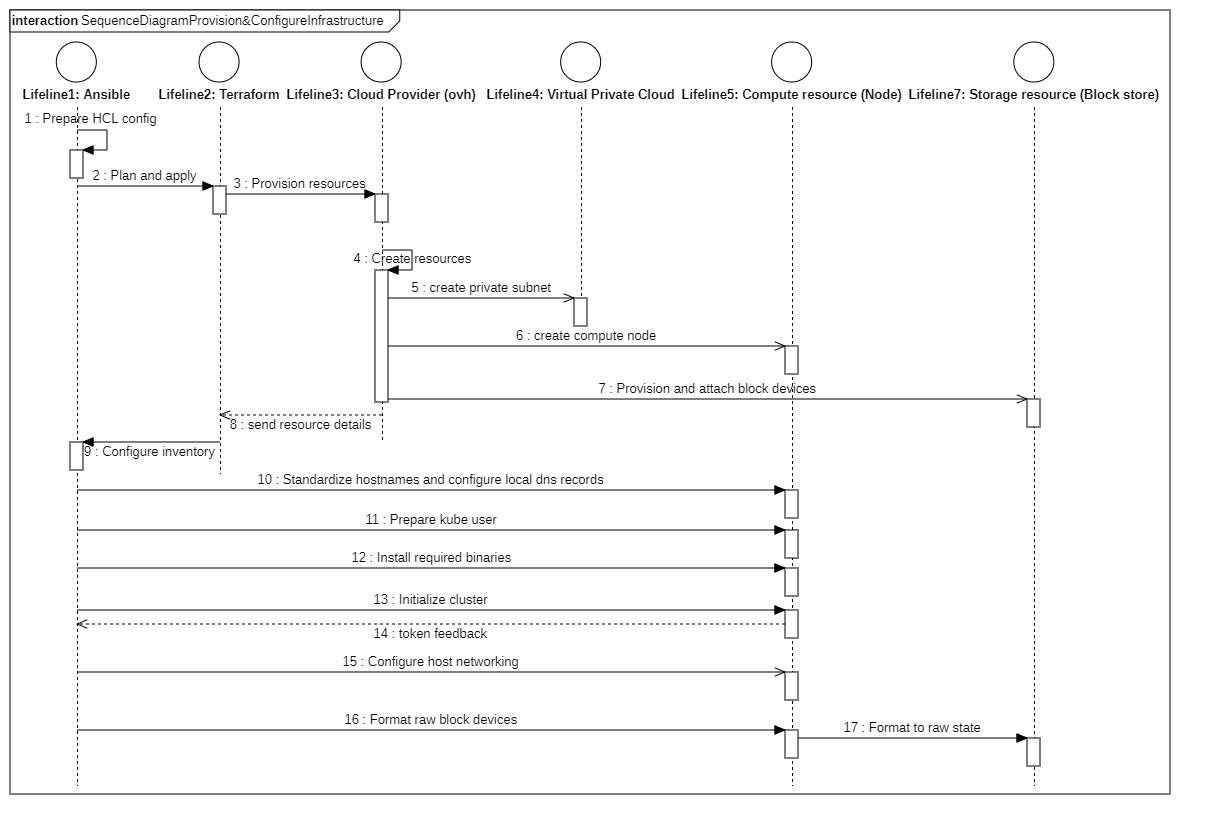
\includegraphics[width=1.0\textwidth,angle=00]{assets/f16.png}
\caption{Sequence diagram for infrastructure setup}
\label{fig:Sequence diagram for infrastructure setup}
\end{figure}


The infrastructure setup process begins with the user initiating an Ansible playbook. The playbook performs several tasks: firstly, it sets up the host machine for Terraform, which then communicates with the OVH API to provision the necessary resources such as virtual machines, block storage volumes, and network interfaces.

Terraform applies any required configurations to these resources. Subsequently, Ansible takes over by configuring the provisioned resources, including package installations, network configurations, and software application setups.

Finally, if everything functions as expected, a notification is sent via an Office 360 webhook channel to notify the devSecOps team that the infrastructure setup process is complete and the system is ready for use.

\subsection{Resource provisioning and infrastructure setup}

The following is a composite diagram for provisioning and setting up the infrastructure. It shows the interaction between the infrastructure as code tools ansible and terraform. 

\begin{figure}[H]\centering
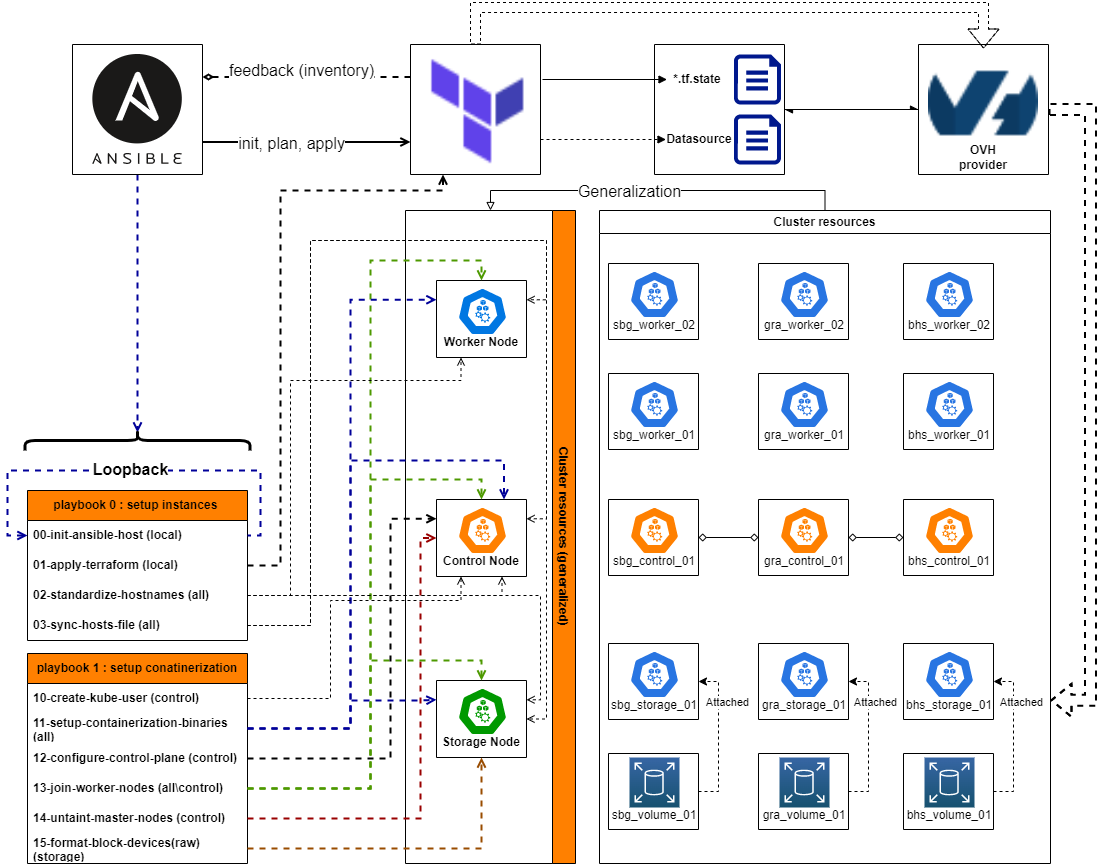
\includegraphics[width=1.0\textwidth,angle=00]{assets/f19.png}
\caption{Orchestrated cluster setup}
\label{fig:Orchestrated cluster setup}
\end{figure}

The ansible playbook begins by setting up prerequisites on each node, including tasks like disabling swap, firewall, and installing required packages.

It then initializes the first node as a master and joins the others as secondary masters, configuring necessary files, certificates, and keys for the Kubernetes control plane.

Afterward, the playbook proceeds to join the worker nodes by providing them with the appropriate configuration information. 

Once all nodes are part of the cluster, networking is established using the Calico CNI plugin, deploying the required network configuration files and pods for inter-node communication. 

Finally, the playbook handles any additional cluster customizations, such as untainting nodes, formatting block volumes, and adding scripts for seamless namespace and context switching.
\newpage
\section{Initial setup of the backend services }
\subsection{UML design: package diagram for the initial PaaS services setup}

Within the PaaS package, there are three sub-packages: the Kubernetes control plane for orchestration, the layer 4 and 7 load balancers for efficient traffic distribution, cloud appliances like Authelia for secure access control.

Additionally, it includes the distributed storage backend for reliable and scalable storage capabilities.

\begin{figure}[H]\centering
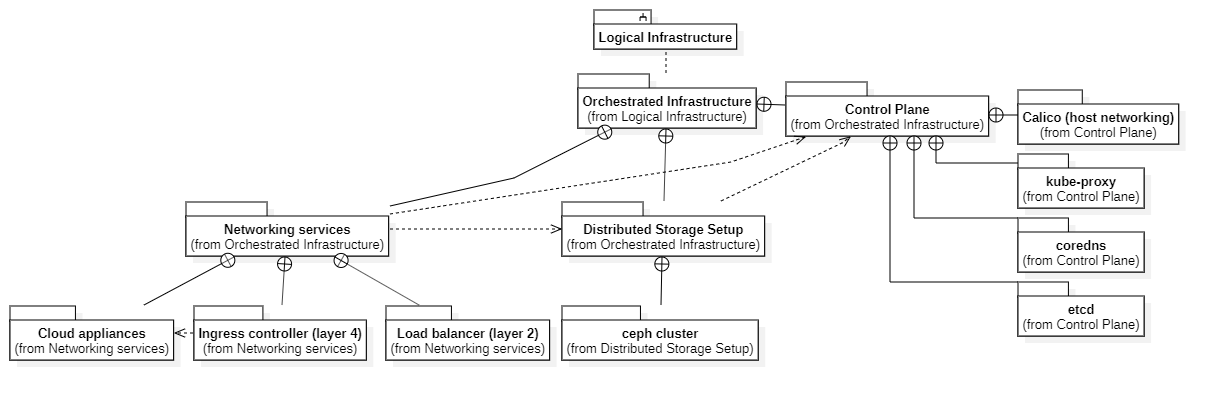
\includegraphics[width=1.0\textwidth,angle=00]{assets/f21.png}
\caption{ Package diagram for the initial PaaS setup }
\label{fig:package diagram for the initial PaaS setup}
\end{figure}

Together, these sub-packages enhance the functionality of the PaaS platform, enabling efficient container management, load balancing, secure access, and robust storage solutions.

\newpage

\subsection{Networking services}

\subsubsection{Overview on the networking services}

As illustrated in the following figure, Traefik, Cert-manager, and MetalLB work together to provide a secure and scalable way to route traffic inside Kubernetes using Services and IngressRoutes.

\begin{figure}[H]\centering
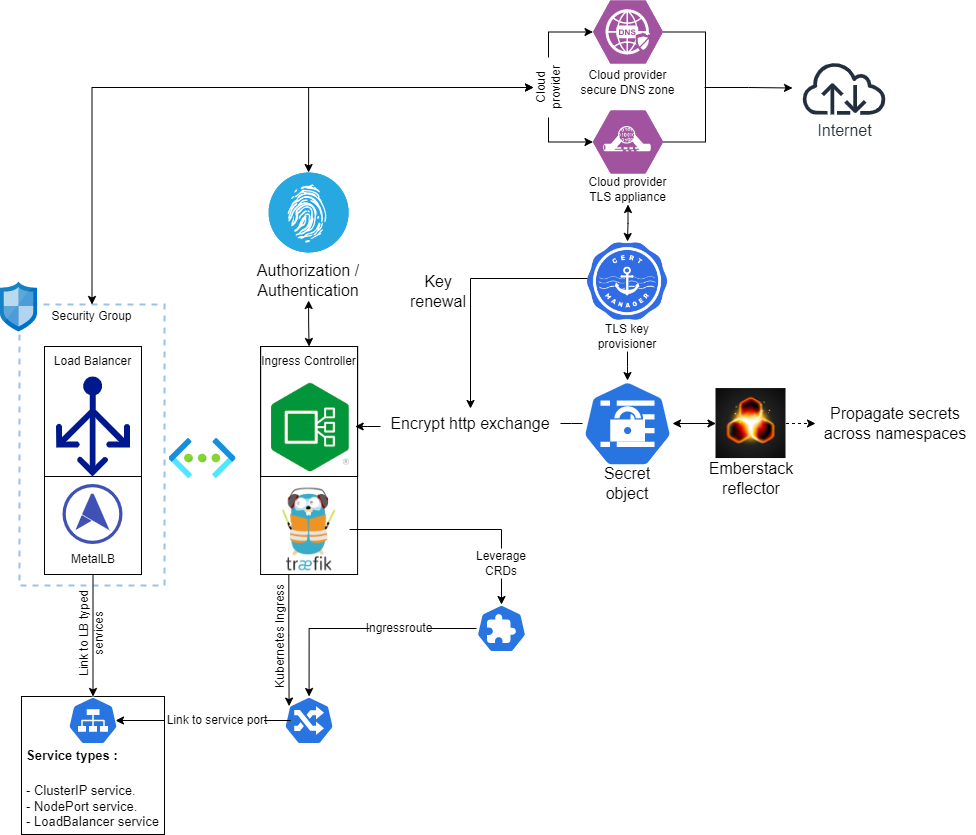
\includegraphics[width=0.85\textwidth,angle=00]{assets/f22.png}
\caption{ Networking services}
\label{fig:Networking services}
\end{figure}

Application workloads are exposed through various types of services, such as ClusterIP, LoadBalancer, and NodePort, for different access scenarios.

Cert-manager acts as a cluster issuer, provisioning TLS certificates through a DNS challenge. It listens to certificate resources, generates valid TLS certificates stored in secrets, and periodically renews them while Emberstack reflector propagates secrets and configmaps across namespaces.

Traffic enters through MetalLB or Traefik for load balancing. Traefik routes traffic to Kubernetes Services linked to configured ingressroutes based on the domain name.

Requests are directed to the appropriate Pods, processed, and responses are sent back via Traefik. TLS termination is mostly handled by Traefik using the generated secrets.

\newpage

\subsubsection{Layer 4 load balancing: network level }

In this level, load balancing is mostly related to the network, IP addresses, network address translation ( NAT ), and packets. 

\begin{enumerate}[label = (\alph*)]

\item Using the built in Kubernetes capability, NodePort services : The NodePort Service exposes a deployment or a set of pods by mapping a specific port on each node in the cluster to the port of the service. 
This allows external clients to access the service by connecting to any of the nodes in the cluster.

\item Using metalLB for load balancing : LoadBalancer services 
MetalLB is used to provide network load balancing for services running in the cluster. This is a sample service of the "LoadBalancer" type: 

\begin{figure}[H]\centering
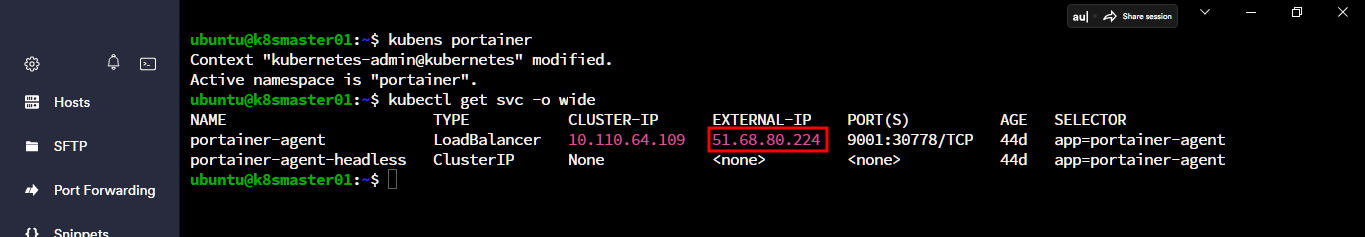
\includegraphics[width=1.0\textwidth,angle=00]{assets/f23.png}
\caption{LoadBalancer service }
\label{fig:LoadBalancer}
\end{figure}

\end{enumerate}


\subsubsection{Secret provisioning and propagation:}

\subsubsubsection{TLS secret provisioning:}

In order to provide secure HTTPS communications between clients and the deployed workloads, valid TLS certificates need to be provisioned from our provider tls appliances. Our tool of choice is cert-manager.

Cert-manager provides us with a powerful and flexible way to manage TLS certificates in Kubernetes, enabling automatic provisioning and renewal of certificates from various certificate authorities, namely: "OVH Cloud Provider" and "Cloudflare".

By automating certificate management, cert-manager helps improve the security and reliability of our Kubernetes services, while reducing the operational burden of manual certificate provisioning and management.

\subsubsubsection{Secret propagation}

Emberstack Reflector, an open-source tool that provides a simple and efficient way to propagate Kubernetes secrets and configmaps across multiple namespaces and clusters. We are using it to automatically replicate a secret from a source namespace to one or more targets, ensuring that all applications that require access to the secret can access it easily.

\subsubsection{Layer 7 load balancing: application level }

Traefik, our ingress controller of choice, functions both as a reverse proxy as well as a load balancer for the deployed workloads that are then accessed through secure HTTPS. 

Note that traefik is capable of receiving configurations from the built-in Kubernetes ingress resource. 

Here we have the dashboard of traefik: 

\begin{figure}[H]\centering
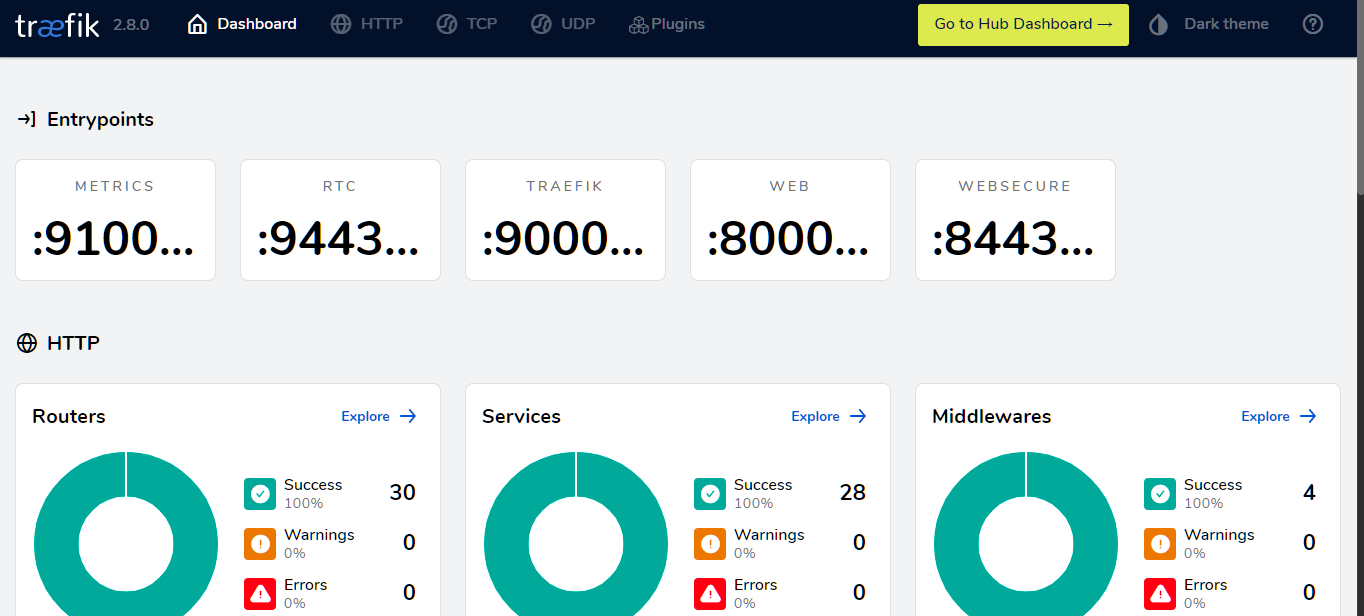
\includegraphics[width=1.0\textwidth,angle=00]{assets/f25.png}
\caption{ Dashboard of traefik }
\label{fig:dashboard of traefik}
\end{figure}

Notice that traefik has multiple entrypoints configured depending on the protocol and the use case. The main entrypoint is websecure. It regulates the HTTPS traffic.  

When Traefik receives an incoming request, it can use the TLS Store to look up the appropriate certificate for the requested domain and use it to encrypt and decrypt traffic. 

Traefik is used in combination with the security layer services to allow for authenticating and authorizing access. The security layer will be discussed in detail further in this report. 

\newpage

\subsection{Authentication and authorization}
\subsubsection{Conceptual overview }

Previously, traefik has been deployed and configured to serve as an ingress controller and load balancer for our platform as a service. Here we discuss how an assortment of components are used in combination with traefik to provide a secure and scalable solution for authentication and authorization. 

The following diagram illustrates the layout of this architecture: 

\begin{figure}[H]\centering
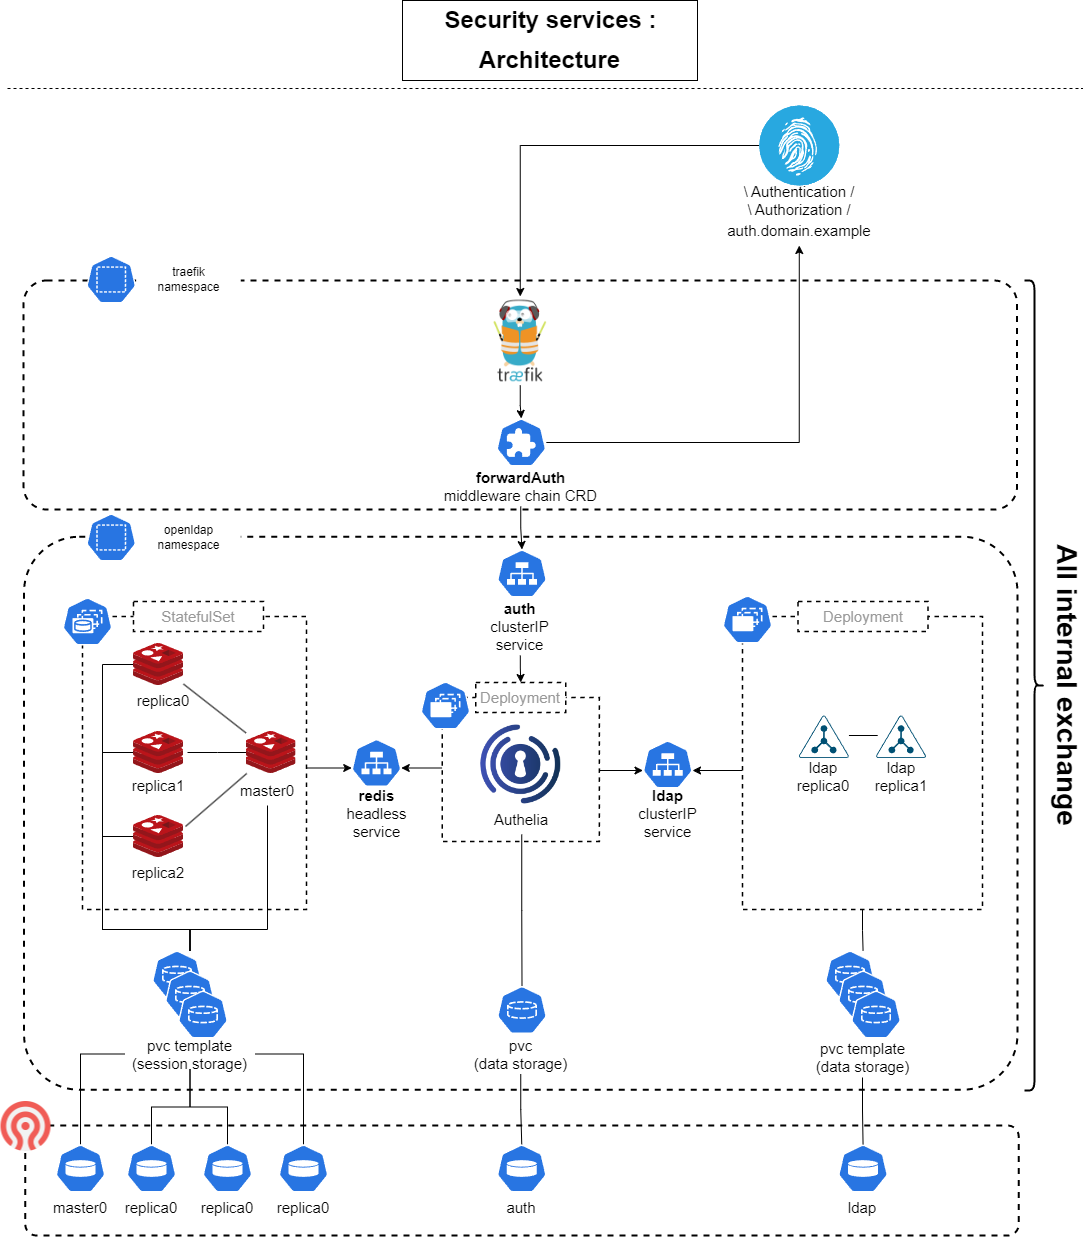
\includegraphics[width=0.9\textwidth,angle=00]{assets/f51.png}
\caption{Conceptual overview }
\label{fig:f51}
\end{figure} 

\newpage

\textbf{Authelia} is used as a forward authentication and authorization controller, which provides an additional layer of security by enforcing authentication and authorization before requests are forwarded to the backend services. Authelia also provides Single Sign-On (SSO) functionality, allowing users to authenticate once and access multiple applications seamlessly.Authelia authenticates users against the OpenLDAP server and authorizes access to resources based on LDAP group membership.  

\textbf{OpenLDAP}, which stores user information and credentials for authentication and authorization purposes, is used as an LDAP server in conjunction with a web interface to facilitate management. 

\textbf{Redis} is used for session storage, which stores user session information to ensure that users remain authenticated and authorized throughout their session. 

\subsubsection{OpenLDAP for access and user management  }

A custom Openldap server is deployed for the purpose of safely and reliably accessing and managing the distributed directories that store information about users, groups, resources. 

The web interface below is deployed and configured to provide secure remote access to the openLDAP server entries, thus allowing management operations. This is achieved using the LDAP base name of the company. Naturally, external direct access to server is prohibited.

\begin{figure}[H]\centering
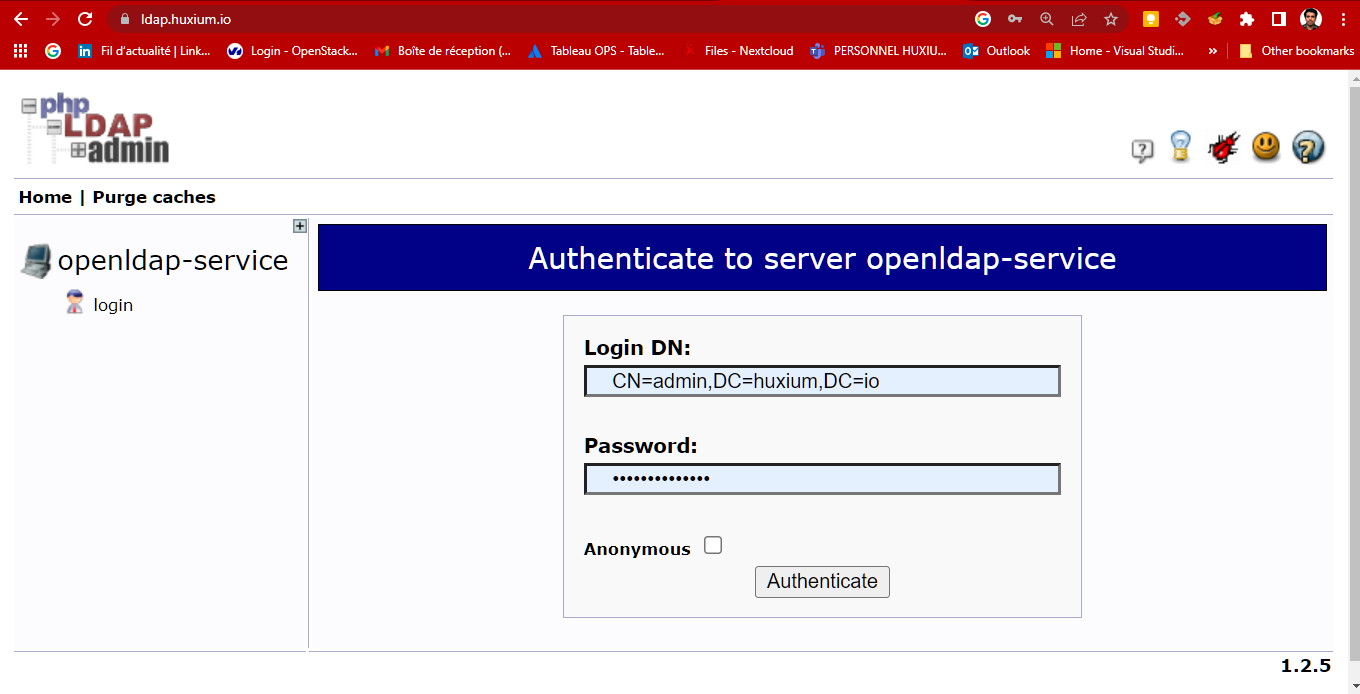
\includegraphics[width=1.0\textwidth,angle=00]{assets/f52.png}
\caption{Figure 52 }
\label{fig:f52}
\end{figure} 

\newpage

\subsubsection{Redis for session storage }

Redis is used with the “auth-middleware” for session storage because Redis is an efficient and highly scalable in-memory data store that can handle high-traffic web applications. 

The following is an overview of the resulting ReplicaSet for Redis: 

\begin{figure}[H]\centering
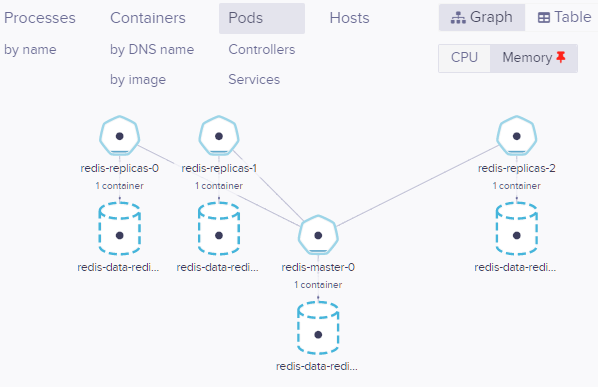
\includegraphics[width=1.0\textwidth,angle=00]{assets/f53.png}
\caption{Figure 53 }
\label{fig:f53}
\end{figure}

The ReplicaSet contains 4 pods with a persistent volume each. The pod hierarchy is as follows: One master pod with the read/write privilege and three replicas with read-only access.

Only internal access is allowed. This is achieved using the following services: 

\begin{itemize}[label={--}]
\item redis-master.openldap.svc.cluster.local for read/write operations (port 6379) 
\item redis-replicas.openldap.svc.cluster.local for read-only operations (port 6379) 
\end{itemize}

\newpage

\subsubsection{Authelia for single sign-on }

Authelia is put in place to provide a single sign-on experience and fine-grained access control for applications and services running on the cluster.

The following is an overview of the deployed resources: 
\begin{figure}[H]\centering
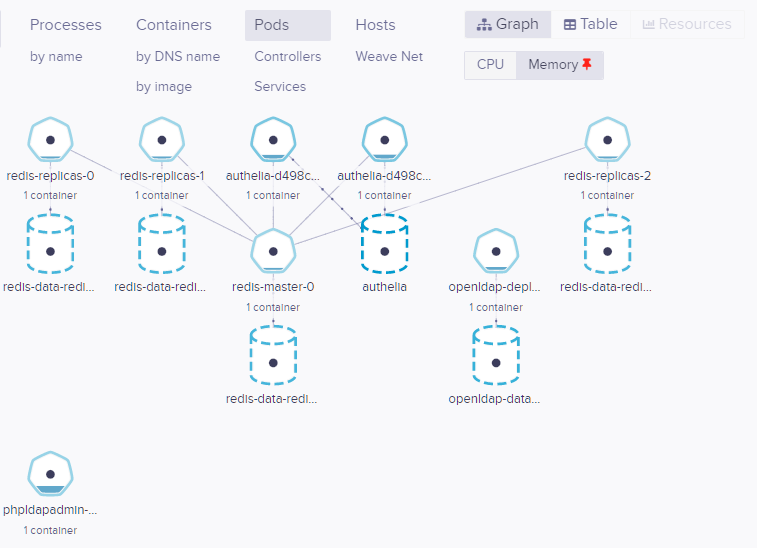
\includegraphics[width=1.0\textwidth,angle=00]{assets/f54.png}
\caption{Deployed resources}
\label{fig:f54}
\end{figure}

This diagram features the following elements: 

\begin{itemize}[label={--}]
\item A deployment of authelia configured with a horizontal pod autoscaler.  
\item The replicated Redis cluster to stora session data. 
\item The openLDAP server that houses user credentials. 
\end{itemize}

Each of these workloads has volumes attached to it in order to persist data. 

\newpage

\subsubsection{The authentication gateway in action }

Forward authentication with Traefik means that incoming requests to a service are first authenticated by Authelia before being forwarded to the service.

A middleware chain is used to authenticate and authorize HTTP requests based on various headers. These headers can include the Authorization header, session cookies, and other custom headers that contain authentication information. 

The following figure shows the authentication portal as seen by an external user: 
\begin{figure}[H]\centering
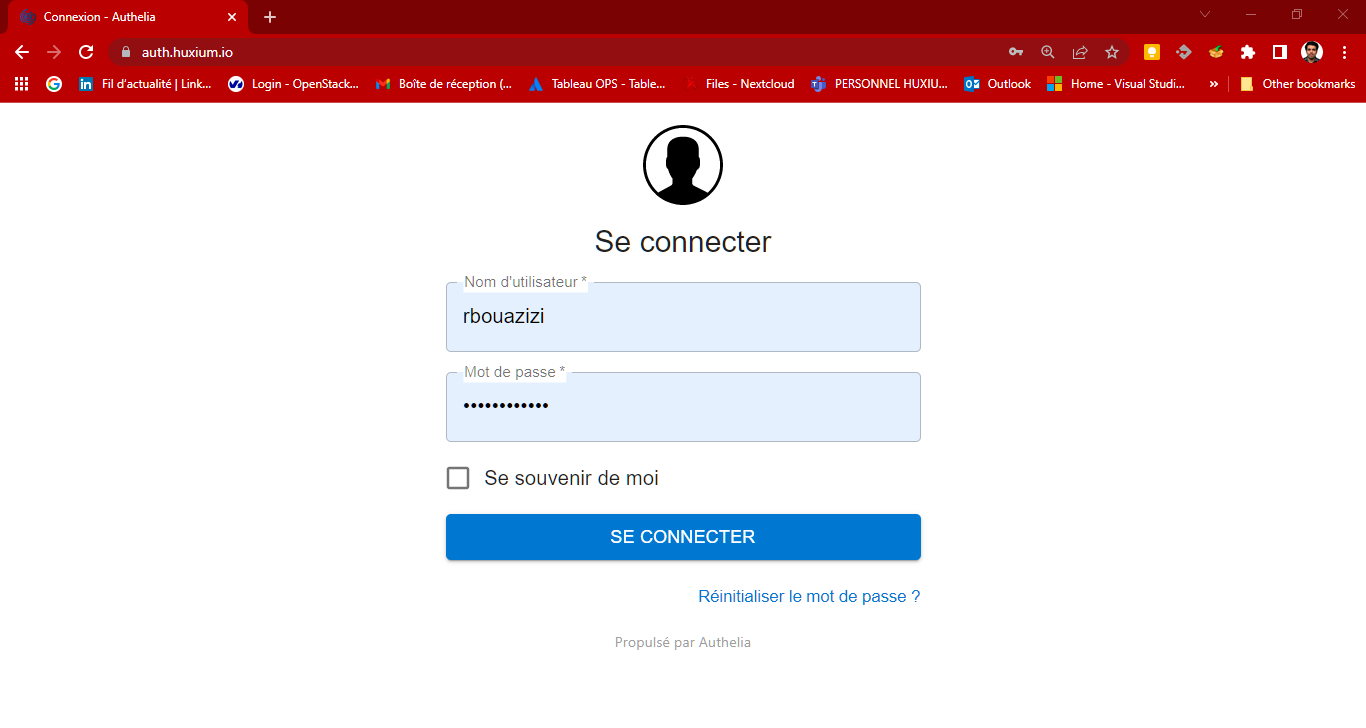
\includegraphics[width=1.0\textwidth,angle=00]{assets/f55.png}
\caption{Authentication portal}
\label{fig:f55}
\end{figure}

The access flow works as follows: 
\begin{itemize}[label={--}]
\item The user sends a request to access a protected resource. 
\item  Traefik receives the request and forwards it to Authelia. 
\item  Authelia authenticates the user against the OpenLDAP server and checks the user's group membership to determine whether access is authorized. 
\item  If the user is authenticated and authorized, Authelia sets up a session for the user and sends a token to Traefik. 
\item  Traefik receives the token and sets it as a cookie in the user's browser for subsequent requests. 
\item  For subsequent requests, Traefik checks the cookie for a valid token and forwards the request to the backend service if the token is valid. Otherwise, the user is redirected to the authentication page.  
\end{itemize}

\newpage

\subsection{Distributed storage backend}

\subsubsection{Architectural overview on storage}

Distributed persistent storage is important for running stateful applications such as databases that require durable storage. In our context, the ability to store data persistently across multiple nodes in a cluster is implemented using the following architecture: 

\begin{figure}[H]\centering
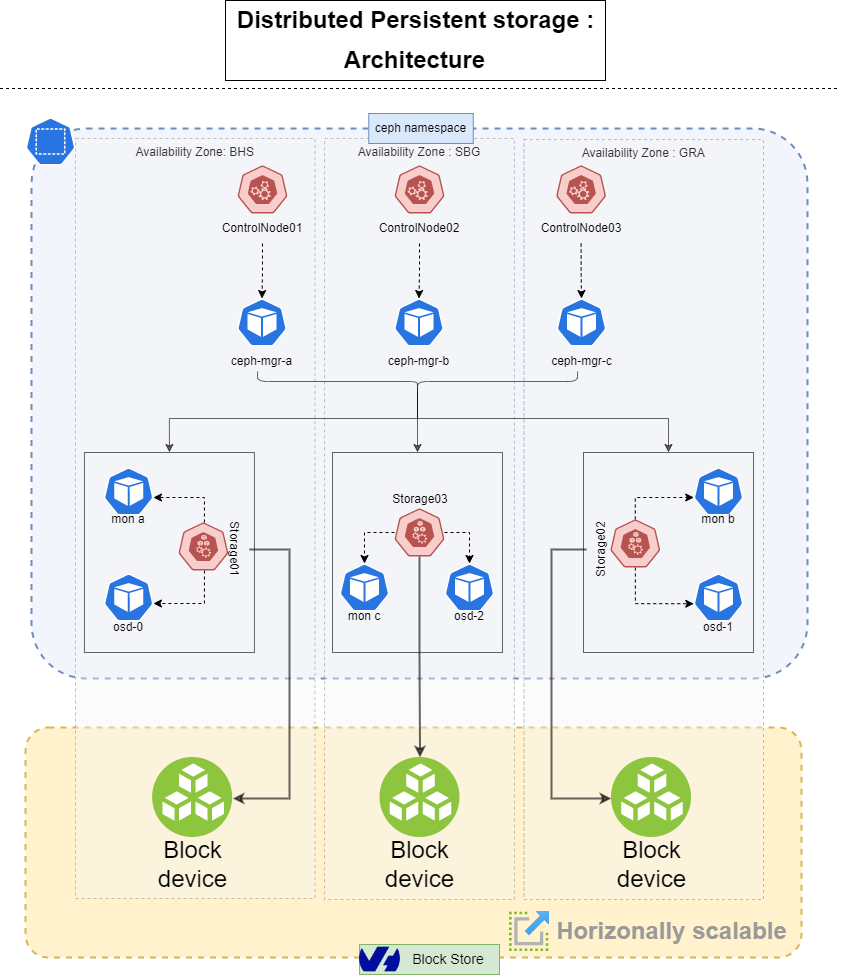
\includegraphics[width=0.78\textwidth,angle=00]{assets/f26.png}
\caption{Architectural overview on storage}
\label{fig:Architectural overview on storage}
\end{figure}

The figure above illustrates a highly scalable storage architecture using “Ceph”. As mentioned in the infrastructure provisioning chapter, in each region, we have created a dedicated storage instance to which a disk the raw format has been attached. The number of disks attached to each node is infinitely scalable and only dependent on the specs of the instance to which it is attached. Furthermore, the size of each disk can be scaled up by the cloud provider. That being said, the number of instances is itself theoretically infinitely scalable. And thus, both horizontal and vertical scalability is achieved. 

\subsubsection{Ceph as a storage provider for kubernetes }

“Ceph”, our storage provider includes several components, such as monitors, managers, OSDs (object storage daemons), and MDSs (metadata servers). These components work together to provide distributed storage.

Ceph is configured such that it will use every raw block device attached to the storage nodes. These block devices join the storage pool.

For each storageNode, the operator spawns an OSD (Object Storage Daemon) which is a storage node that stores objects, e.g., the basic units of data.

Using the ingress controller, a dashboard for “ceph” is exposed and allows for observability on the storage backend: 
\begin{figure}[H]\centering
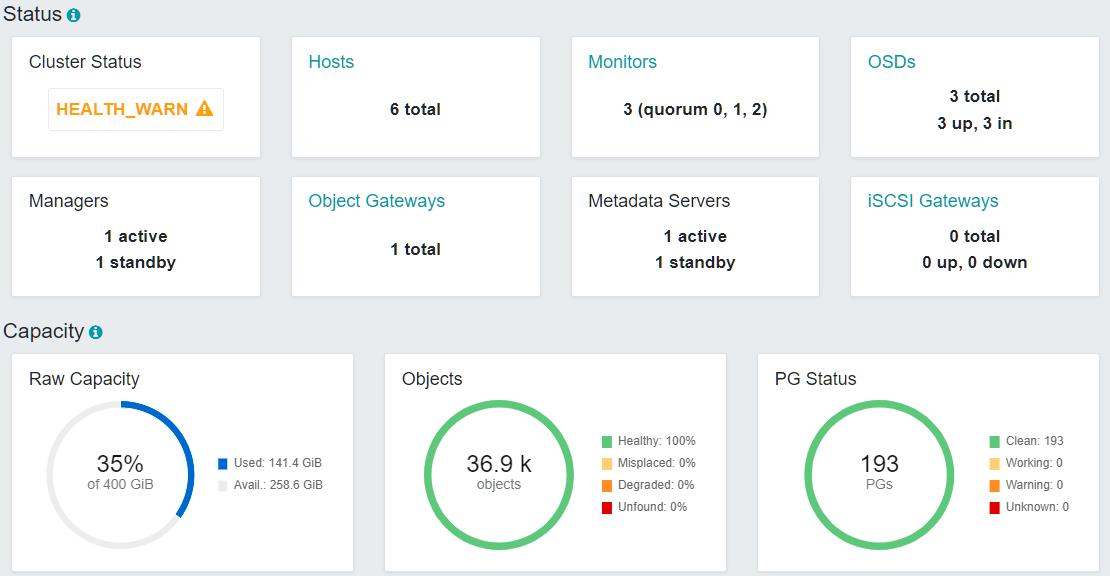
\includegraphics[width=1.0\textwidth,angle=00]{assets/f29.png}
\caption{Ceph Dashboard }
\label{fig:Ceph Dashboard }
\end{figure}

\newpage

\subsubsubsection{The filesystem storage mode: }

In order to leverage the filesystem storage mode, we have declared a StorageClass that specifies the storage parameters for the file system, such as the size of the file system and the type of file system (e.g., ext4 or xfs).

Using the Persistent Volume Claim object, the CSI provisioner will dynamically provision a volume from the CephFS file system and mount it to the pod.

As shown by the figure below, CephFS provides built-in redundancy and fault tolerance, ensuring that data is always available even in the event of hardware failures. 
\begin{figure}[H]\centering
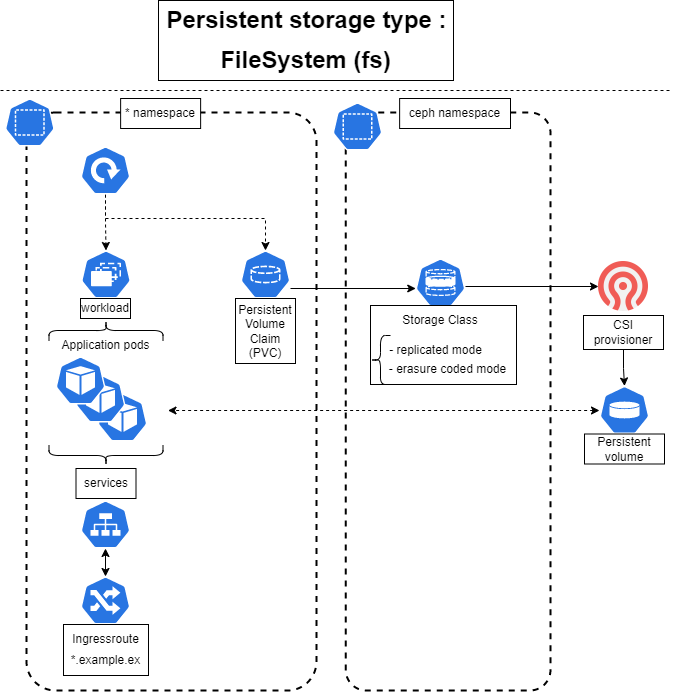
\includegraphics[width=1.0\textwidth,angle=00]{assets/f31.png}
\caption{Filesystem Storage}
\label{fig:Filesystem Storage}
\end{figure}
\newpage
\subsubsubsection{The object storage mode: }

It stores data as objects, rather than as files or blocks. This allows applications to store and retrieve large amounts of unstructured data in a highly available and fault-tolerant manner. Ceph Object Storage exposes an S3-compatible API. It is mainly used to cache backup data inside the cluster before being sent to S3 buckets on the cloud.

The procedure to provision object store buckets is as follows: 

\begin{enumerate}[label = (\arabic*)]
    \item First we create the CephObjectStore CRD that starts the RGW (RadosGateWay) service in the cluster with an S3 API. 
    \item Next, an object store StorageClass is created. It contains such as the reclaimPolicy and the objectStore to which it is linked. 
    \item Finally, for every bucket we desire to create, we either use the S3 API to converse with the RGW or we declare an ObjectBucketClaim which will then be resolved to a bucket. 
\end{enumerate}


This procedure is summarized by the following figure: 

\begin{figure}[H]\centering
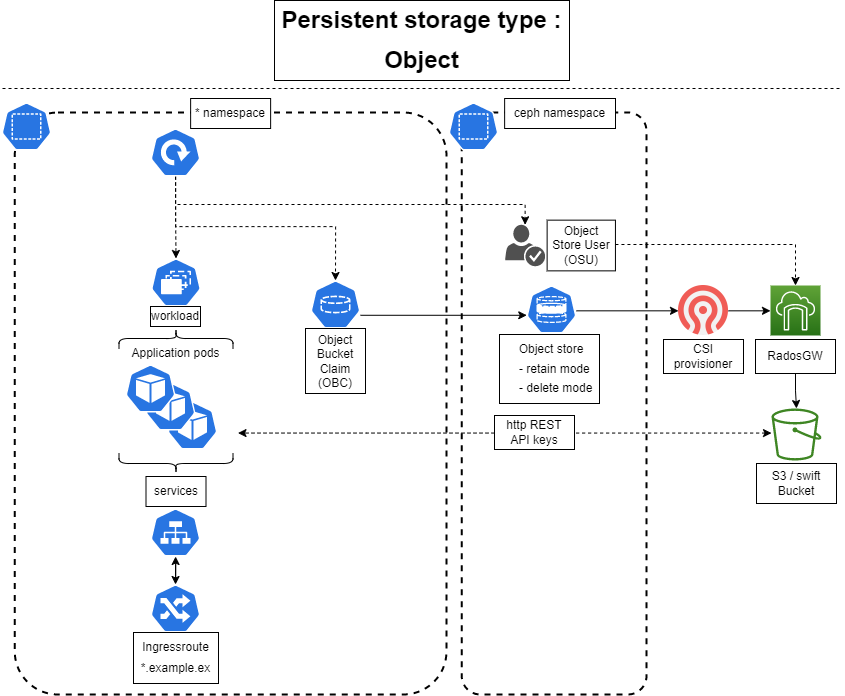
\includegraphics[width=1.0\textwidth,angle=00]{assets/f32.png}
\caption{Object Storage mode }
\label{fig:Object Storage mode}
\end{figure}
\newpage
\subsubsubsection{The block storage mode: }

Ceph Block Storage exposes a block device interface. But due to the very nature of a containerized environment, we are not using this capability. The following is a summary on the procedure to provision block devices using ceph: 

\begin{figure}[H]\centering
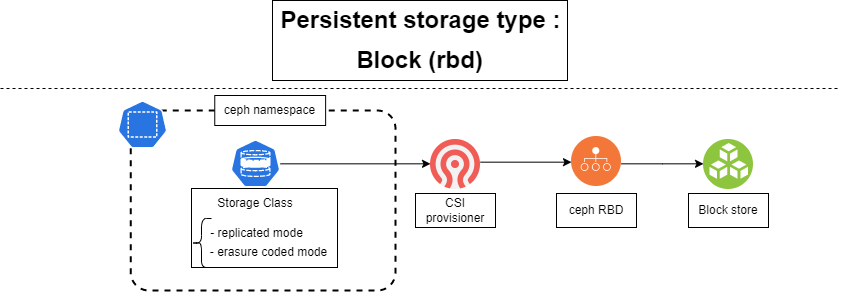
\includegraphics[width=1.0\textwidth,angle=00]{assets/f33.png}
\caption{Block Storage Procedure}
\label{fig:Block Storage Procedure}
\end{figure}

This provides dynamic and on-demand provisioning of block storage volumes to the applications running on Kubernetes.


\subsubsection{Summary on the deployed storage capabilities: }

The following diagram provides an overview on the storage capabilities of ceph : 
\begin{figure}[H]\centering
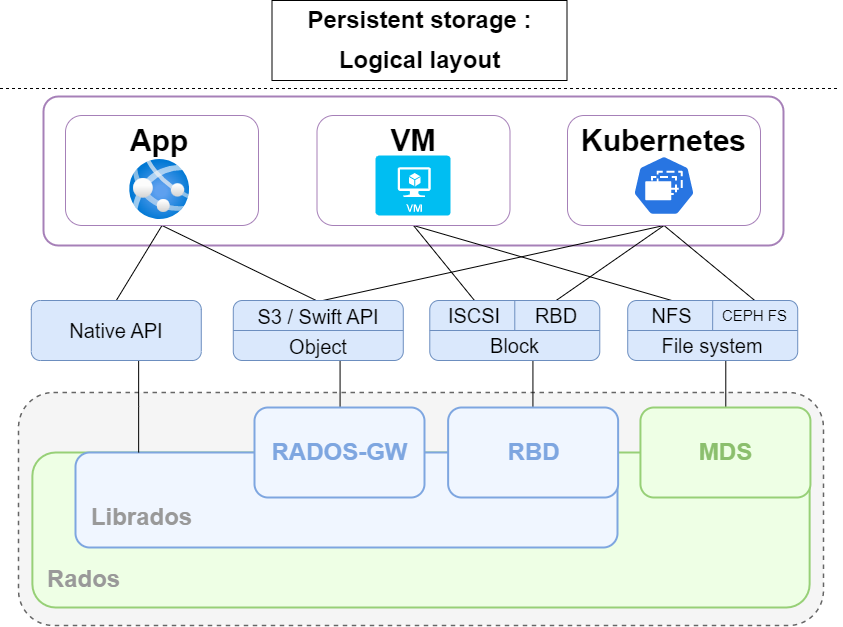
\includegraphics[width=0.8\textwidth,angle=00]{assets/f30.png}
\caption{Storage capabilities Diagram}
\label{fig:f30}
\end{figure}
\section{Conclusion}

This chapter provides a comprehensive overview of the preliminary setup of our Platform-as-a-Service (PaaS) infrastructure. We reviewed and maintained the existing infrastructure, ensuring a solid foundation for our PaaS platform.

The carefully crafted cloud architectural design guarantees scalability and robustness. Efficient resource provisioning strategies optimize utilization. The preliminary infrastructure setup establishes a secure and reliable PaaS environment. 

Additionally, we successfully implemented critical backend services such as networking, load balancing, TLS provisioning, distributed storage, and authentication services.

With the completion of this chapter, we can proceed confidently to the subsequent stages of the project, further enhancing the capabilities of our PaaS infrastructure.